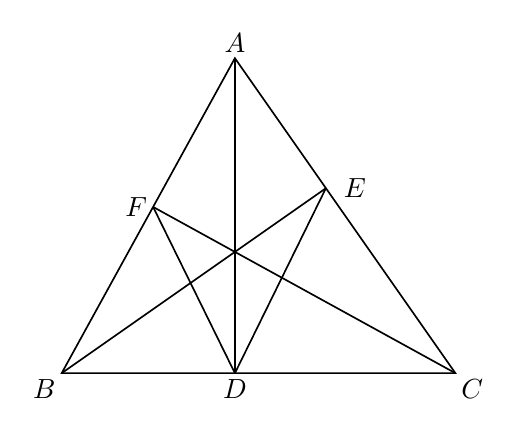
\begin{tikzpicture}[x=1cm,y=1cm,font=\normalsize,
 geometry edge/.style={solid,line width=.6pt},
 geometry mark/.style={solid,line width=.6pt},
 geometry label/.style={font=\normalsize,inner sep=2pt}]
\coordinate (A) at (2.2,4.0);
\coordinate (B) at (0,0);
\coordinate (C) at (5.0,0);
\coordinate (D) at (2.2,0);
\coordinate (E) at (3.3557,2.349);
\coordinate (F) at (1.1612,2.1113);
\coordinate (H) at (2.2,1.54);
\draw[geometry edge] (A)--(B)--(C)--cycle;
\draw[geometry edge] (A)--(D);
\draw[geometry edge] (B)--(E);
\draw[geometry edge] (C)--(F);
\draw[geometry edge] (D)--(F);
\draw[geometry edge] (D)--(E);
\node[geometry label,above] at (A) {$A$};
\node[geometry label,below left] at (B) {$B$};
\node[geometry label,below right] at (C) {$C$};
\node[geometry label,below] at (D) {$D$};
\node[geometry label,right,xshift=1.5mm] at (E) {$E$};
\node[geometry label,left] at (F) {$F$};
\end{tikzpicture}
